\documentclass[aspectratio=169]{beamer}
\usepackage[utf8]{inputenc}
\usepackage[T1]{fontenc}
\usepackage[magyar]{babel}
\usepackage{hyperref}
\usepackage{biblatex}
\usepackage{csquotes}
\usepackage{graphicx}
\usepackage{amsmath}
\usepackage{amssymb}

% Acous-optics Bragg Diffraction Interaction of sound and light
% Doppler-shift Acousto optic devices

\setbeamertemplate{navigation symbols}{}
%\setbeamertemplate{footline}[frame number]
\setbeamertemplate{caption}{\insertcaption}

\usetheme{Madrid}
\usecolortheme{default}
\usefonttheme[onlymath]{serif}
\renewcommand{\figurename}{}
\newcommand{\framet}{\frametitle{\secname{} - \subsecname}}

\begin{document}
\title{Akusztooptika}
\subtitle{Bragg-diffrakció, fény és hang interakció,\\Doppler-effektus, akusztooptikai berendezések}
\author{Készítette: Illés Gergő}
\date{2023. május 02.}
\begin{frame}
\maketitle
\end{frame}

\begin{frame}
\frametitle{Tartalomjegyzék}

\begin{columns}
\column{.90\textwidth}
\tableofcontents
\end{columns}
\end{frame}

\section{Bragg-diffrakció}
\begin{frame}
\frametitle{\secname{} - Akusztooptika mint kifejezés}
\begin{itemize}
\item Optikai közegek törésmutatója megváltoztatható mechanikai ráhatással
\item Használhatunk ultrahangot
\item Akusztooptika: A hanghullámok által előidézett optikai tulajdonságváltozás vizsgálata
\item Felhasználása: optikai modulátorok, eltérítők, frekvencia modulátor, spektrum analizátor
\end{itemize}
\end{frame}
\begin{frame}
\frametitle{\secname}
\begin{columns}
\column{.6\textwidth}
\begin{itemize}
\item A röntgensugarak kristályokban történő diffrakcióját 1913-ban publikálták.
\item A jelenséget William Henry Bragg és fia William Lawrence Bragg fedezte fel és később róluk nevezték el.
\item A diffrakciót a rácsok egyes fősíkjairól visszaverődő sugarak interferenciája okozza.
\item Bragg-diffrakcióról beszélünk az akusztooptika témakörében is, de ilyenkor a diffrakció más okból jön létre
\end{itemize}
\column{.4\textwidth}
\begin{figure}
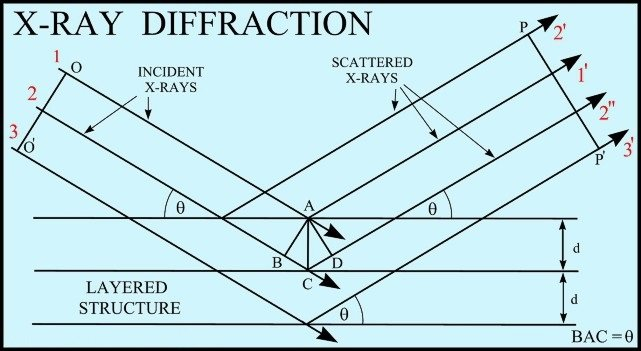
\includegraphics[width=.9\textwidth]{xrd6.jpg}
\caption{A Bragg diffrakció illusztrációja}
\end{figure}
\end{columns}
\end{frame}


\begin{frame}

\begin{columns}
\column{.5\textwidth}
\begin{itemize}
\item Az akusztooptikában a kristály rácsperiódusánál jóval nagyobb hullámhosszakat használnak.
\item Ezen források általában lézerek a látható-, vagy ahhoz közeli tartományban sugároznak.
\item $n\lambda=2d\sin(\theta)$ - Röntgen diffrakció
\item $\lambda=2n\Lambda\sin(\alpha)$ - Akusztooptikai diffrakció
\end{itemize}
\column{.5\textwidth}
\begin{figure}
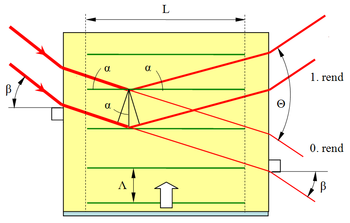
\includegraphics[width=.95\textwidth]{bragg-diff.png}
\caption{Akusztooptikai Bragg diffrakció}
\end{figure}
\end{columns}
\end{frame}

\begin{frame}
\begin{figure}
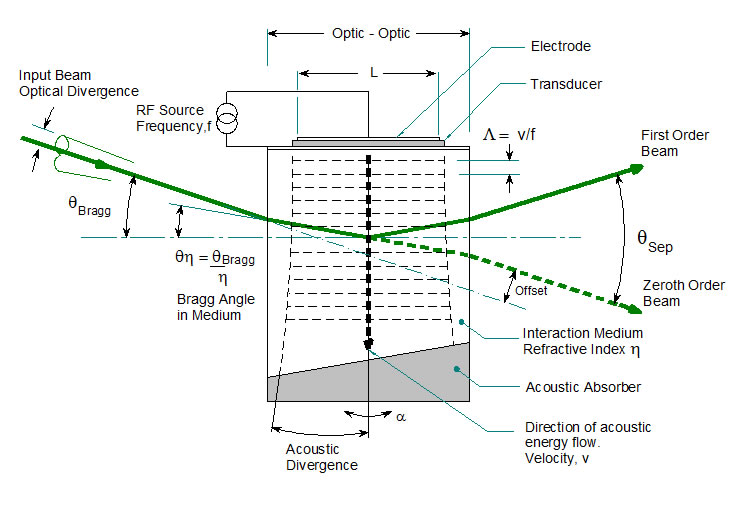
\includegraphics[width=.8\textwidth]{isomet.jpg}
\end{figure}
\end{frame}

\begin{frame}
\begin{itemize}
\item Definiálhatunk egy akusztooptikai tényezőt (merit): $\mathcal{M}=\dfrac{p^2n^6}{\rho v^3}$\\ahol $p$: elaszto-optikai együttható, $n$: törésmutató, $v$: hangsebesség, $\rho$:~tömegi~sűrűség
\item A törésmutató változása:$\Delta n_0=\sqrt{\frac{1}{2}\mathcal{M}I_s}$, ahol $I_s$ a hang intenzitása
\end{itemize}
\end{frame}


\begin{frame}
\begin{itemize}
\item A Bragg-cella reflexiója: $r_\pm=\pm i\,r_0\,\mathrm{sinc}\left[(2k\sin(\theta)\mp q)\frac{L}{2\pi}\right]\cdot\mathrm{exp}(\pm i\Omega t)$
\item A $\pm$ két komponenst jelöl
\item $r_+$ a Bragg upshifted, $r_-$ pedig Bragg downshifted reflexió
\item $r_+$ akkor maximális, amikor $2k\sin(\theta)=q$
\end{itemize}
\begin{figure}
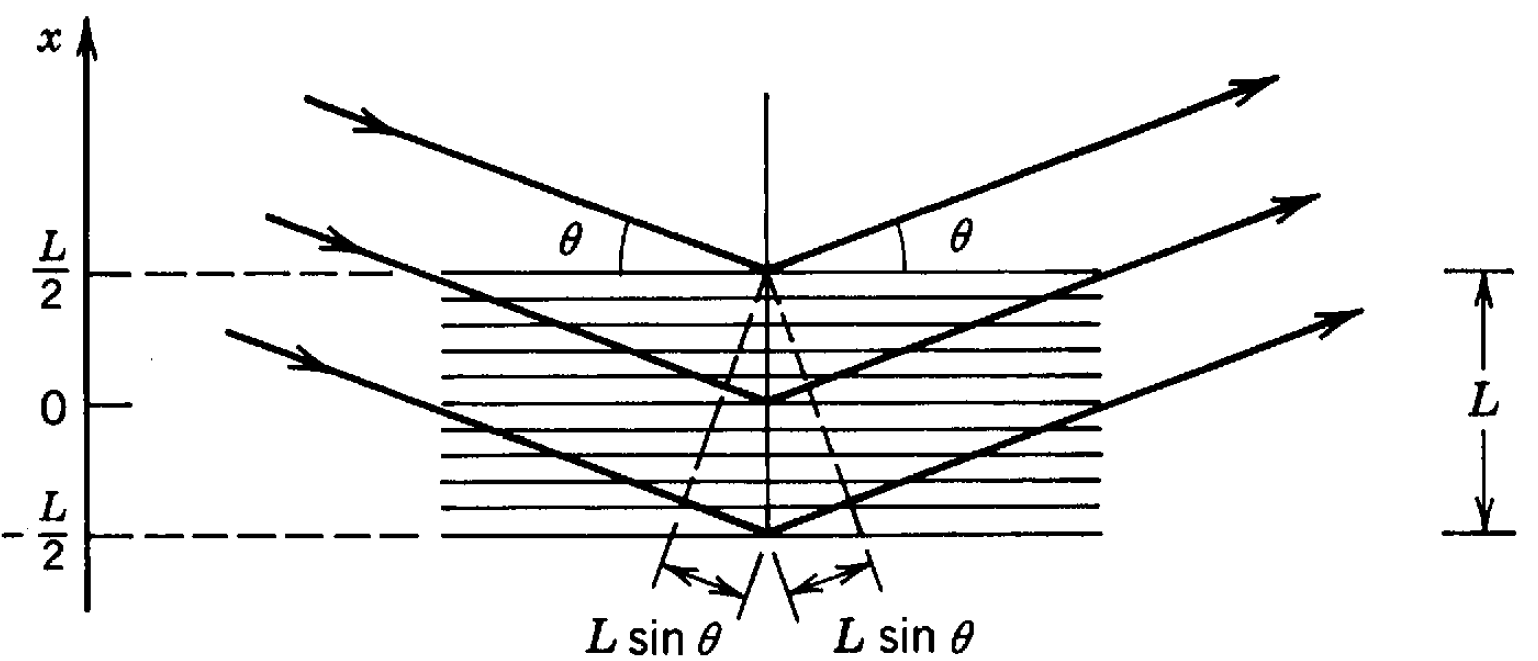
\includegraphics[width=.6\textwidth]{reflexio.png}
\caption{Reflexió periodikusan anizotróp közegben}
\end{figure}
\vspace*{-30pt}
\end{frame}

\begin{frame}
\begin{columns}
\column{.6\textwidth}
\begin{itemize}
\item $r_+$ maximális ha $2k\sin(\theta)=q$.
\item $q=\frac{2\pi}{\Lambda}$ valamint $k=\frac{2\pi}{\lambda}$.
\item Visszahelyettesítve megkapjuk a Bragg feltételt: $\sin(\theta_B)=\frac{\lambda}{2\Lambda}$.
\item A reflexió csak a ezen $\theta_B$ szög közelében van jelen.
\item Amikor $\sin(\theta)-\sin(\theta_B)=\frac{\lambda}{2L}$ a reflexió megszűnik.
\end{itemize}
\column{.4\textwidth}
\begin{figure}
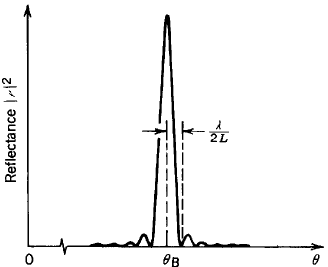
\includegraphics[width=\textwidth]{sinc.png}
\caption{Reflektált intenzitás $\theta$ függvényében}
\end{figure}
\end{columns}
\end{frame}

\section{Doppler eltolódás}
\begin{frame}
\frametitle{\secname}
\begin{itemize}
\item A felületekről visszavert fény frekvenciája megváltozik
\item Ez egy Doppler eltolásként is felfogható
\item Az $r_+$ reflexióé $\omega+\Omega$ az $r_-$-é pedig $\omega-\Omega$
\end{itemize}
\begin{columns}
\column{.5\textwidth}
\begin{figure}
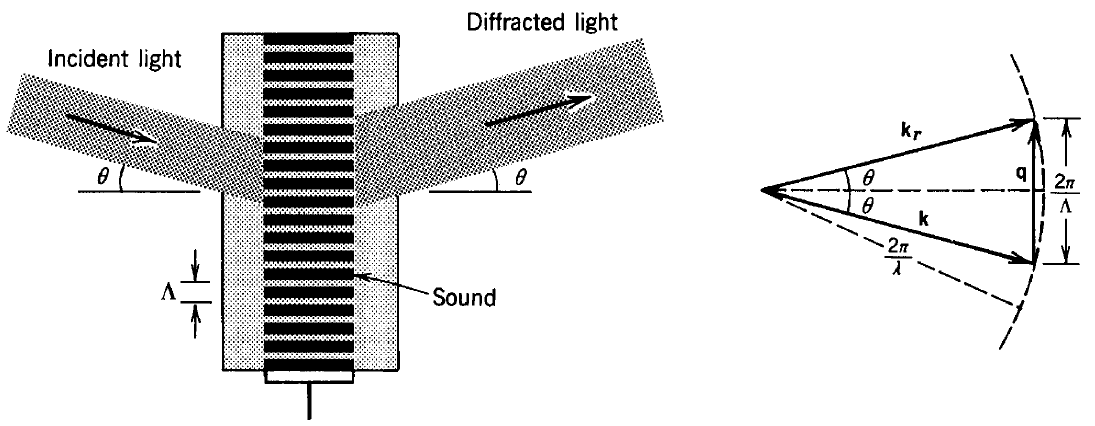
\includegraphics[width=.95\textwidth]{refp.png}
\caption{Bragg upshift}
\end{figure}
\column{.5\textwidth}
\begin{figure}
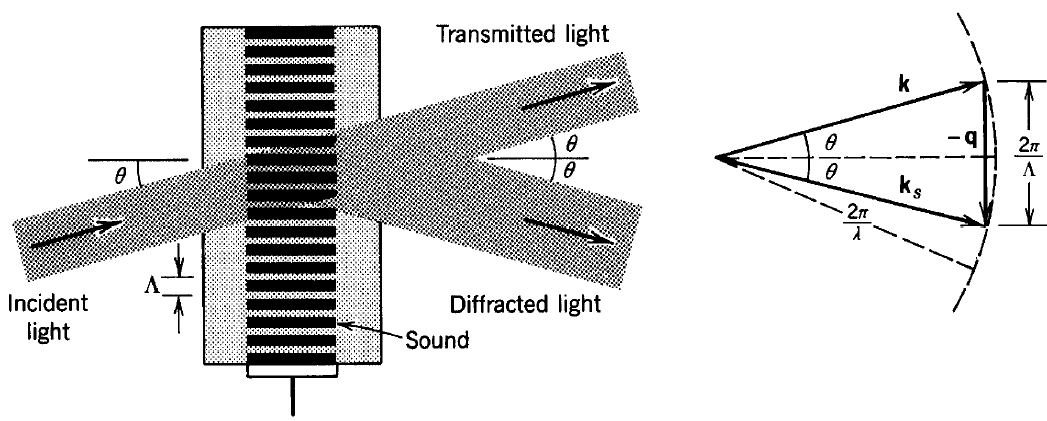
\includegraphics[width=.95\textwidth]{refm.png}
\caption{Bragg downshift}
\end{figure}
\end{columns}
\end{frame}
\section{Kvantumos értelmezés}
\begin{frame}
\frametitle{\secname}
\begin{columns}
\column{.68\textwidth}
\begin{itemize}
\item A kvantummechanika szerint a fény elemi csomagokban terjed
\item A fény kvantuma a foton
\item Az anyagi közegben terjedő hullámok szintén kvantáltak
\item A mechanikai rezgések kvantuma a fonon
\item A reflexió felfogható egy fonon-foton kölcsönhatásként
\item $\hbar k_r = \hbar k + \hbar q$
\end{itemize}
\column{.32\textwidth}
\begin{figure}
\raggedright
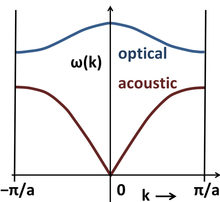
\includegraphics[width=.95\textwidth]{diat_phonon.png}
\caption{Diszperziós reláció}
\end{figure}
\end{columns}
\end{frame}
\section{Egyéb esetek}
\subsection{Fókuszált nyaláb síkhullámokról való visszaverődése}
\begin{frame}
\frametitle{\subsecname}
\begin{figure}
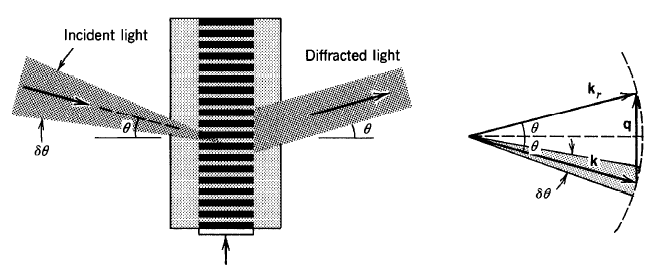
\includegraphics[width=.85\textwidth]{beam-planar.png}
\caption{Fókuszált nyaláb síkhullámról való reflektálódása}
\end{figure}
\end{frame}
\subsection{Fókuszált nyaláb görbült frontról való visszaverődése}
\begin{frame}
\frametitle{\subsecname}
\begin{figure}
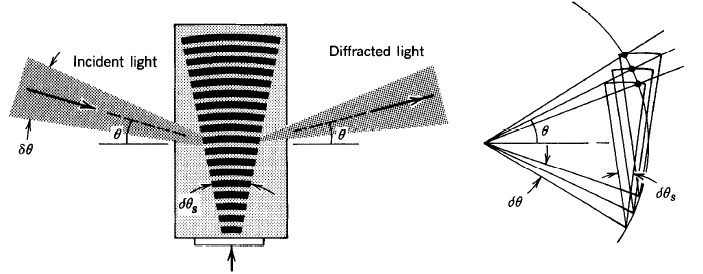
\includegraphics[width=.85\textwidth]{beam-spherical.png}
\caption{Fókuszált nyaláb görbült frontról való reflektálódása}
\end{figure}
\end{frame}

\section{Akusztooptikai eszközök}
\begin{frame}
\frametitle{\secname}
Az akusztooptikai eszközök előnyei:
\begin{enumerate}
\item Az eszközök sokkal gyorsabbak mint a hagyományos optikai eszközök.
\item Alacsony zaj, kevés hibát adnak a méréshez.
\item Jó hatásfok, 100 $\frac{W}{cm^2}$-es hangintenzitás mellett 19\%-os reflexió.
\item Jól integrálható komplex rendszerekbe.
\end{enumerate}
\end{frame}

\subsection{Modulátor}
\begin{frame}
\framet
\begin{figure}
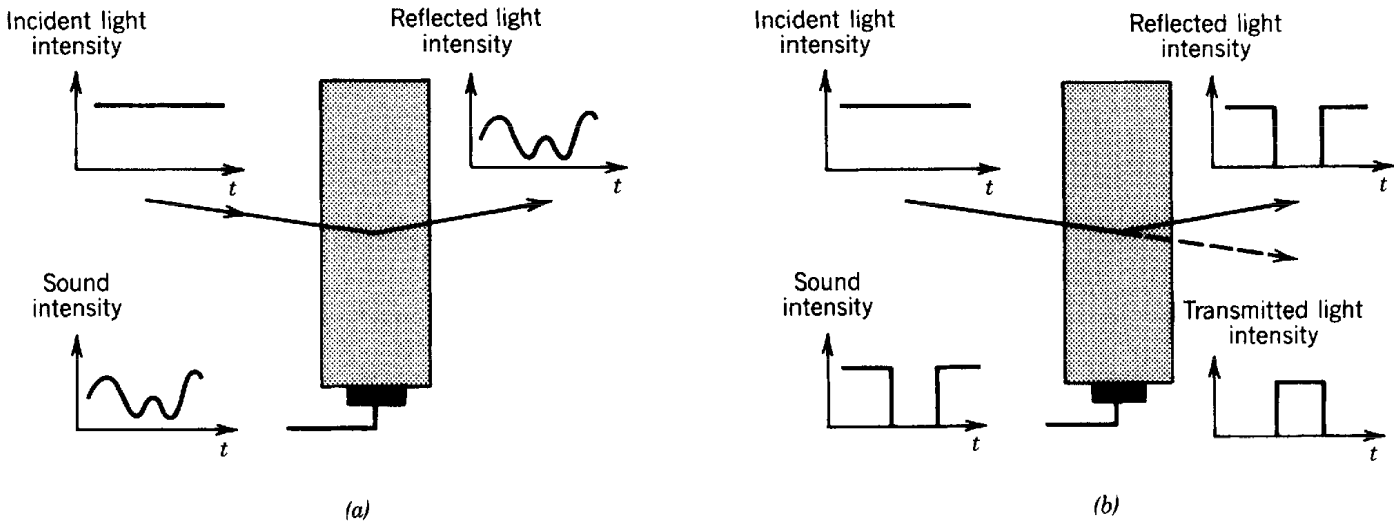
\includegraphics[width=\textwidth]{mod.png}
\caption{\hspace*{20pt}Modulátor\hspace*{180pt}Kapcsoló}
\end{figure}
\end{frame}
\subsection{Szkenner}
\begin{frame}
\framet
\begin{columns}
\column{.2\textwidth}
\begin{itemize}
\item $\Delta\theta=\dfrac{\lambda}{v_s}f_{mod}$
\end{itemize}
\column{.8\textwidth}
\begin{figure}
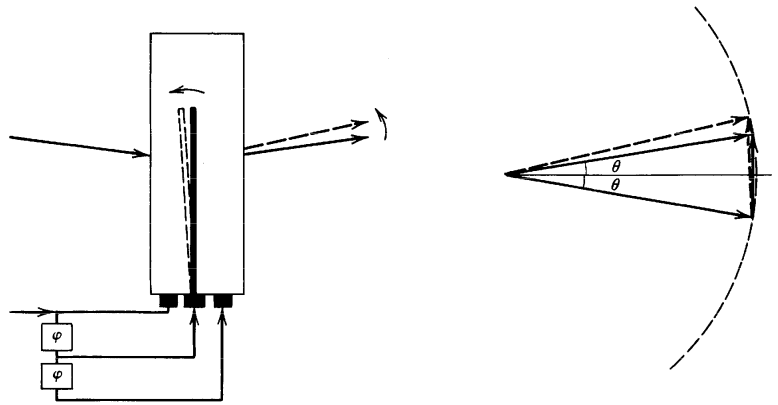
\includegraphics[width=.9\textwidth]{scanner.png}
\caption{Akusztooptikai szkenner}
\end{figure}
\end{columns}
\end{frame}

\subsection{Jelszétválasztás}

\begin{frame}
\framet
\begin{columns}
\column{.5\textwidth}
\begin{figure}
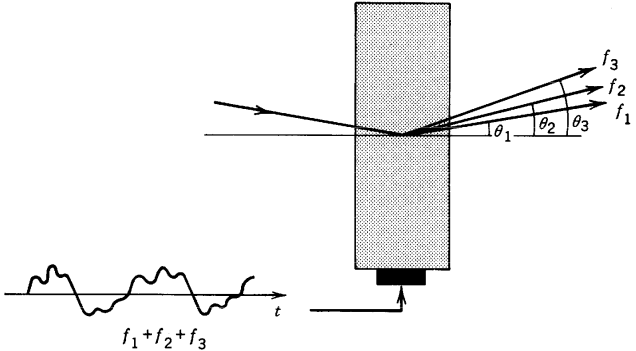
\includegraphics[width=\textwidth]{ic1.png}
\end{figure}
\column{.5\textwidth}
\begin{figure}
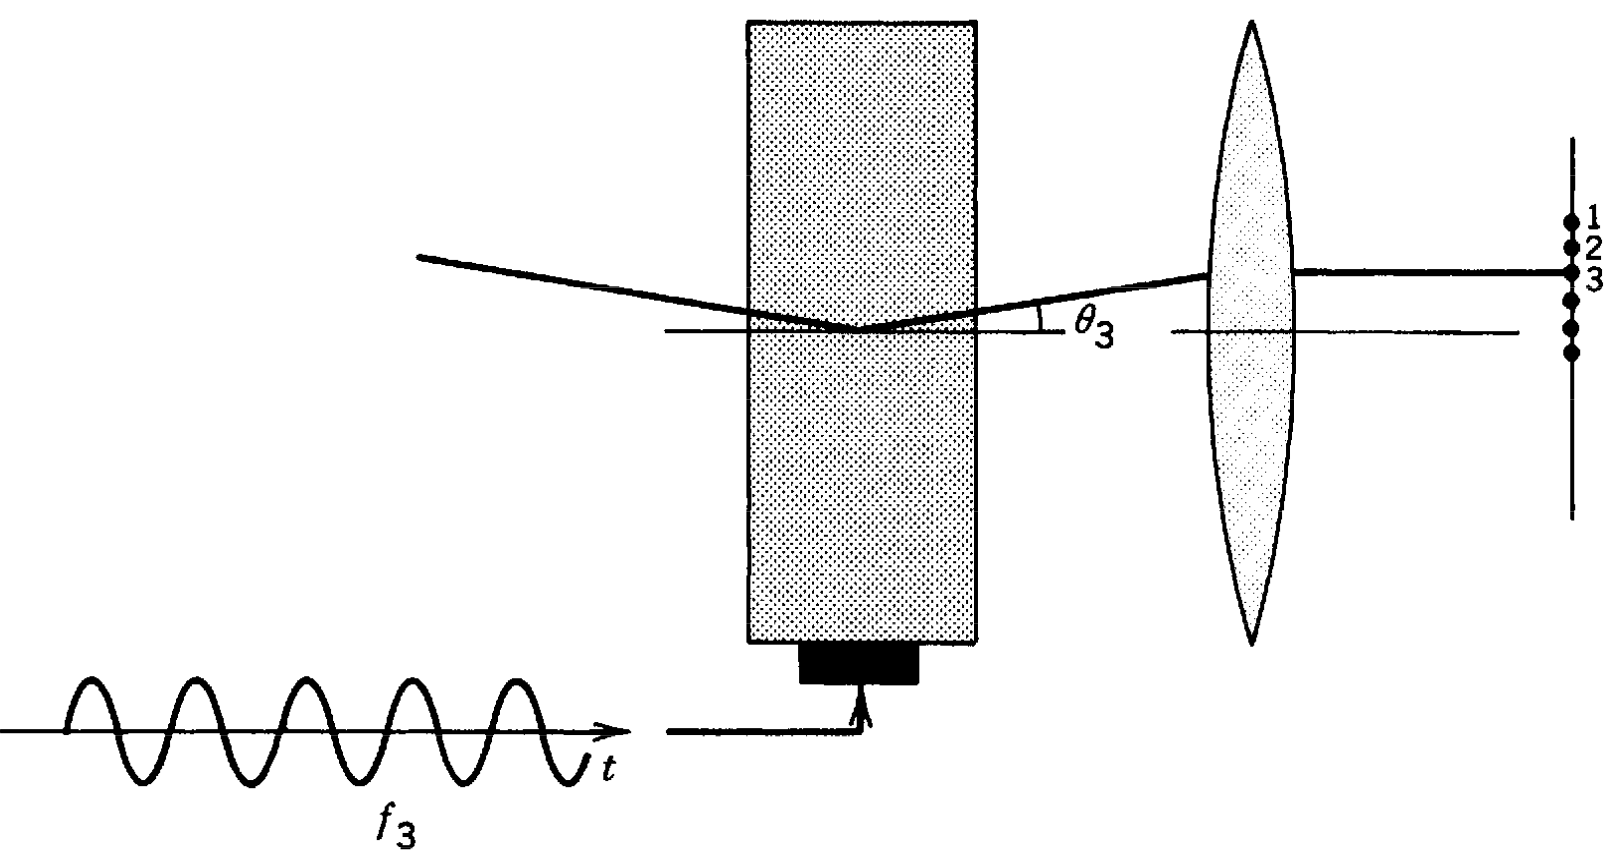
\includegraphics[width=\textwidth]{ic2.png}
\end{figure}
\end{columns}
\centering
Akusztooptikai jelszétválasztó
\end{frame}

\section{Hivatkozások}
\begin{frame}
\frametitle{\secname}
\begin{thebibliography}{99}
\footnotesize
\bibitem{saleh-teich} Saleh, Teich: Fundamentals of Photonics Chapter 20.
\bibitem{physopen} \url{https://physicsopenlab.org/2018/01/18/bragg-diffraction/}
\bibitem{fizpedia} \url{https://fizipedia.bme.hu/index.php/Akusztooptikai_f\%C3\%A9nydiffrakci\%C3\%B3_vizsg\%C3\%A1lata}
\bibitem{isomet} \url{https://isomet.com/acousto_optics.html}
\end{thebibliography}
\end{frame}
\end{document}